\documentclass[tikz,border=12pt]{standalone}
\usepackage[T1]{fontenc}
\usepackage{tgheros}
\usepackage{sfmath}
\usepackage{amsmath}
\usepackage{fontawesome5}
\usepackage{tikz}
\usetikzlibrary{arrows.meta,positioning,shapes.geometric,fit,backgrounds,calc}
\usepackage{xcolor}

\renewcommand{\familydefault}{\sfdefault}

% Harvard Crimson & ETH Zurich Academic Semantic Palette
\definecolor{harvardcrimson}{HTML}{A51C30}
\definecolor{ethdarkblue}{HTML}{1F407A}
\definecolor{ethblue}{HTML}{215CAF}
\definecolor{ethpetrol}{HTML}{007A87}
\definecolor{ethbronze}{HTML}{B87333}
\definecolor{ethslate}{HTML}{475569}
\definecolor{cardbg}{HTML}{F8FAFC}
\definecolor{cardborder}{HTML}{CBD5E1}

\begin{document}
\begin{tikzpicture}[
  font=\sffamily,
  >=Stealth,
  box/.style={
    draw=cardborder,
    fill=cardbg,
    rounded corners=5pt,
    line width=0.9pt,
    text width=3.45in,
    minimum height=2.45in,
    inner sep=9pt,
    align=left,
    anchor=north,
    text=ethdarkblue
  }
]

  % Top Title Banner
  \node[draw=ethdarkblue, fill=ethdarkblue!5, rounded corners=5pt, line width=1pt, text width=8.50in, inner sep=7pt, align=center] (title) at (4.25in, 0) {
    {\normalsize\bfseries\color{ethdarkblue}\faIcon{microchip}\;\; HARDWARE-TRIGGERED METROLOGY TOPOLOGY}\\[2pt]
    {\scriptsize\color{ethslate}Escaping Software Timestamp Delusions via Logic Analyzer GPIO Toggles and Shunt Current Probes}
  };

  % Left Card: The Machine Under Test
  \node[box] (dut) at (0, -0.65in) {
    {\small\bfseries\color{ethdarkblue}\faIcon{server}\; Physical AI Machine Under Test}\\[3pt]
    {\scriptsize\bfseries\color{ethslate}Arduino UNO Q Dual-Brain Platform}\\[6pt]
    \textbf{\color{ethblue}1. Sensor Frame Interrupt (GPIO 1):}\\[1pt]
    {\tiny Toggled inside camera driver ISR on DMA start.}\\[4pt]
    \textbf{\color{ethbronze}2. MPU Inference Emit (GPIO 2):}\\[1pt]
    {\tiny Toggled in Linux kernel upon writing RPMSG mailbox.}\\[4pt]
    \textbf{\color{ethpetrol}3. MCU Enforcement Veto / Pass (GPIO 3):}\\[1pt]
    {\tiny Toggled inside FreeRTOS 1 kHz ISR on CBF evaluation.}\\[4pt]
    \textbf{\color{harvardcrimson}4. Inverter Gate Drive Out (PWM Pins):}\\[1pt]
    {\tiny Direct hardware timer registers driving MOSFET bridge.}
  };

  % Right Card: External Test Equipment (Positioned with 1.30in gap)
  \node[box, draw=ethpetrol, fill=ethpetrol!5] (scope) at (4.75in, -0.65in) {
    {\small\bfseries\color{ethpetrol}\faIcon{chart-line}\; External Ground-Truth Metrology}\\[3pt]
    {\scriptsize\bfseries\color{ethslate}Multi-Channel Logic Analyzer \& Oscilloscope}\\[6pt]
    \textbf{\color{ethblue}CH 1 (Digital):} Transduction Pulse $\to$ True $t_{\text{transduce}}$\\[3pt]
    \textbf{\color{ethbronze}CH 2 (Digital):} Proposal Generation $\to$ True $t_{\text{inference}}$\\[3pt]
    \textbf{\color{ethpetrol}CH 3 (Digital):} MCU Permission $\to$ True $t_{\text{enforce}}$\\[3pt]
    \textbf{\color{harvardcrimson}CH 4 (Analog):} Current Shunt $\to$ Motor Coil $L/R$ Rise Time\\[6pt]
    \rule{0.95\linewidth}{0.3pt}\\[4pt]
    {\scriptsize\textbf{\color{ethdarkblue}Guaranteed Result: Zero Operating System Jitter.}}
  };

  % Connecting Probes with Clear Spacing
  \draw[->, line width=1.2pt, ethblue] ($(dut.north east) + (0, -0.45in)$) -- ($(scope.north west) + (0, -0.45in)$)
    node[midway, font=\sffamily\bfseries\tiny, fill=white, draw=ethblue!40, rounded corners=2pt, inner sep=2pt, text=ethblue] {Probe 1: Ingest};

  \draw[->, line width=1.2pt, ethbronze] ($(dut.north east) + (0, -0.95in)$) -- ($(scope.north west) + (0, -0.95in)$)
    node[midway, font=\sffamily\bfseries\tiny, fill=white, draw=ethbronze!40, rounded corners=2pt, inner sep=2pt, text=ethbronze] {Probe 2: Inference};

  \draw[->, line width=1.2pt, ethpetrol] ($(dut.north east) + (0, -1.45in)$) -- ($(scope.north west) + (0, -1.45in)$)
    node[midway, font=\sffamily\bfseries\tiny, fill=white, draw=ethpetrol!40, rounded corners=2pt, inner sep=2pt, text=ethpetrol] {Probe 3: Enforce};

  \draw[->, line width=1.2pt, harvardcrimson] ($(dut.north east) + (0, -1.95in)$) -- ($(scope.north west) + (0, -1.95in)$)
    node[midway, font=\sffamily\bfseries\tiny, fill=white, draw=harvardcrimson!40, rounded corners=2pt, inner sep=2pt, text=harvardcrimson] {Probe 4: Coil Current};

\end{tikzpicture}
\end{document}
